%% %% %% %%
%%
%% Parte B de la práctica
%%
%% %% %% %%

\documentclass[../procedimientos.tex]{subfiles}
\graphicspath{{\subfix{../../images/}}}

\begin{document}
\clearpage
\subsection{Parte B}
\begin{em}
  Diseñar mediante la programación estructurada la implementación de una unidad 
  lógica-aritmética binaria de dos palabras de 4 bits, como se muestra en la 
  siguiente tabla:
\end{em}
\begin{table}[H]
  \centering
  \begin{tabular}{ccc|c|c}
    \hline
    $s_1$ & $s_0$ & $c_i$ & Aritmético ($M=0$) & Lógico ($M=1$)\\
    \hline
    0 & 0 & 0 & $A$ & $A \cdot B$\\
    0 & 0 & 1 & $A+1$ & $A + B$\\
    0 & 1 & 0 & $A+B$ & $\n{A}$\\
    0 & 1 & 1 & $A+B+1$ & $A \oplus B$\\
    1 & 0 & 0 & $A+\n{B}$ & $\nt{A + B}$\\
    1 & 0 & 1 & $A+\n{B}+1(A-B)$ & $\nt{A \cdot B}$\\
    1 & 1 & 0 & $A-1$ & $B$\\
    1 & 1 & 1 & $A$ & $\n{A} \cdot B$
  \end{tabular}
  \caption{Tabla de verdad del funcionamiento de la ALU}
  \label{tab:ul_func}
\end{table}

Para comenzar esta sección, fue importante hacer uso de las siguientes tablas 
(poroporcionadas en el planteamiento de la práctica) para llevar a cabo la 
impelemntación de la unidad aritmética.
\begin{table}[H]
  \centering
  \begin{tabular}{p{1cm}p{1cm}p{1cm}|p{2cm}|p{2cm}|p{6cm}}
    \hline
    \multicolumn{3}{p{3cm}|}{\textbf{Selector}} & \textbf{Salida Ni} & 
    \textbf{Función} & \textbf{Descripción}\\
    \hline
    $s_1$ & $s_0$ & $c_i$ & $N_i$ & $F$\\
    \hline
    0 & 0 & 0 & 0 & $A$ & Transferir $A$\\
    0 & 0 & 1 & 0 & $A + 1$ & Incrementar $A$\\
    0 & 1 & 0 & $B$ & $A + B$ & Sumar o agregar $B$ a $A$\\
    0 & 1 & 1 & $B$ & $A + B + 1$ & Suma con acarreo\\
    1 & 0 & 0 & 0 & $A + \n{B}$ & Agregar $C_1(B)$ a $A$\\
    1 & 0 & 1 & 0 & $A + \n{B} + 1$ & Agregar $C_2(B)$ a $A$\\
    1 & 1 & 0 & Todos $1$ & $A - 1$ & Decrementar $A$\\
    1 & 1 & 1 & Todos $1$ & $A$ & Transferir $A$\\
  \end{tabular}
  \caption{Tabla de verdad del funcionamiento de la UL}
  \label{tab:ua_func}
\end{table}

Simplificando un poco la información brindada por la tabla anterior,se tiene 
que:
\begin{table}[H]
  \centering
  \begin{tabular}{cc|c}
    \hline
    $s_1$ & $s_0$ & $N_i$\\
    \hline
    0 & 0 & 0\\
    0 & 1 & $B$\\
    1 & 0 & $\n{B}$\\
    1 & 1 & $1$
  \end{tabular}
\end{table}

Con lo cual se tiene la expresión:
\begin{align*}
  N_i (s_1 s_0) &= \cancel{\n{s_1} \n{s_0} (0)} + \n{s_1} s_0 (B) + s_1 
  \n{s_0} (\n{B}) + s_1 s_0 (1)\\
  &= \n{s_1} s_0 B + s_1 \n{s_0} \n{B} + s_1 s_0\\
  &= (\n{s_1} s_0 B + s_1 s_0) + (s_1 \n{s_0} \n{B} + s_1 s_0)\\
  &= s_0 (\n{s_1} B + s_1) + s_1 (\n{s_0} \n{B} + s_0)\\
  &= s_0 \cancel{(\n{s_1} + s_1)} (B + s_1) + s_1 \cancel{(\n{s_0}+s_0)}\\
  &= s_0 (B + s_1) + s_1 (\n{B} + s_0)\\
  &= s_0 B  + s_1 \n{B} + s_0 s_1\\
  &= s_0 B  + s_1 \n{B} + s_0 s_1 (B + \n{B})\\
  &= s_0 B  + s_1 \n{B} + s_0 s_1 B + s_0 s_1 \n{B}\\
  &= s_0 B (s_1 + 1)  + s_1 \n{B} (s_0 + 1)\\
  &= s_0 B + s_1 \n{B}
\end{align*}
\begin{equation*}
  \boxed{
    \therefore N_i (s_1 s_0) = s_0 B + s_1 \n{B}
  }
\end{equation*}

Entonces, se contruyó la Unidad Aritmética haciendo uso de cuatro \textit{Full 
Adder}, para los cuales se operó por un lado con $a_i$ y por el otro con el 
resultado de $N_i = s_0 b_i + s_1 \n{b_i}$, tal como se muestra en el 
siguiente fragmento de código.

\begin{lstlisting}[language=VHDL]
-- Implementacion de la Unidad Aritmetica
library ieee;
use ieee.std_logic_1164.all;

entity UA is
	port(
    a,b		:in	std_logic_vector(3 downto 0);
		sel		:in	std_logic_vector(2 downto 0);
		res		:out	std_logic_vector(4 downto 0)
	);
end entity;

architecture Behave of UA is
	component FA is
		port(
			ent	:in	std_logic_vector(2 downto 0);
			res	:out	std_logic_vector(1 downto 0)
		);
	end component;
	
	signal c :std_logic_vector(2 downto 0);
	signal n	:std_logic_vector(3 downto 0);
begin
	n <= (
		(sel(1) and b(3)) or (sel(2) and not b(3)),
		(sel(1) and b(2)) or (sel(2) and not b(2)),
		(sel(1) and b(1)) or (sel(2) and not b(1)),
		(sel(1) and b(0)) or (sel(2) and not b(0))
	);

	op_0	:FA port map(
		ent => (a(0), n(0), sel(0)),
		res(1) => res(0),
		res(0) => c(0)
	);
	
	op_1	:FA port map(
		ent => (a(1), n(1), c(0)),
		res(1) => res(1),
		res(0) => c(1)
	);
	
	op_2	:FA port map(
		ent => (a(2), n(2), c(1)),
		res(1) => res(2),
		res(0) => c(2)
	);
	
	op_3	:FA port map(
		ent => (a(3), n(3), c(2)),
		res(1) => res(3),
		res(0) => res(4)
	);
end;
\end{lstlisting}

Tal como se puede ver, se tienen las entradas $a$ y $b$ (con las cuales se 
operará) y una configuración de selección $sel(3)$, la cual es un vector que 
almacena la entrada de selección mostrada en la Tabla \ref{tab:ua_func}.  Se 
hace uso de una señan $n$ para calcular los valores de las respectivas $N_i$ y 
posteriormente se hace udo de los \textbf{Full Adder} $op\_0$, $op\_1$, 
$op\_2$ y $op\_3$ para conformar el resultado de la operación seleccionada, el 
cual se almacena en una palabra de cinco bits: $res(5)$.

Es importante mencionar que la entrada de selección ya incluye el bit de 
acarrero de entrada, el cual será el bit menos significativo, acorde a lo 
establecido en la Tabla \ref{tab:ua_func}.

Por otra parte, la implementación de la Unidad Lógica fue sumamente más 
sencilla ya que cada caso se traduce a una operación lógica en VHDL. Nada más 
se fijaron los casos basándonos en la Tabla \ref{tab:ul_func} a través de una 
estructura \textit{with-select}.
\begin{lstlisting}[language=VHDL]
-- Implementacion de la Unidad Logica
library ieee;
use ieee.std_logic_1164.all;

entity UL is
	port(
		a,b		:in	std_logic_vector(3 downto 0);
		sel		:in	std_logic_vector(2 downto 0);
		res		:out	std_logic_vector(3 downto 0)
  );
end entity;

architecture Behave of UL is
begin
  with sel select
	res <=
    a and b			  when "000",
    a or b 			  when "001",
    not a				  when "010",
		a xor b 			when "011",
		not (a or b)	when "100",
		not (a and b)	when "101",
    b					    when "110",
		not a and b 	when "111";
end;
\end{lstlisting}

Las entradas se manejan de igual forma que en la \textit{Unidad Aritmética}.  
Sin embargo, para este caso se tiene que la salida no corresponde a 5 bits, 
sin o a 4 bits. Esto debido a que como tal las operaciones lógicas no generan 
un acarreo. Por cada par de bits que se opera, sólo existirá un único bit de 
salida.

Para cumplir con el objetivo de la práctica, fue necesario juntar los módulos 
anteriores dentro de una misma entidad, las cual se denominó \textit{ALU} 
(Unidad Aritmético-Lógica por sus siglas en inglés). Dentro de ella se creó 
una entidad de tipo \textit{UL}, la cual tiene una salida $g$ de 4 bits, y una 
unidad \textit{UA}, la cual tiene una salida $f$ de 5 bits. Las entradas del 
sistema son dos palabras de 4 bits ($a$ y $b$), junto con cuatro entradas de 
selección: las mismas tres mencionadas en las secciones anteriores ($s_1$, 
$s_0$, $c_i$) más una adicional para seleccionar el tipo de operación a 
utilizar ($m$).

Sumado a lo anterior se tuv que implementar una estructura similar a un 
multiplexor pero que permitiera seleccionar una palabra de entre un conjunto 
de dos palabras de 5 bits. Este se implementó de forma muy sencilla haciendo 
uso de la estructura \textit{with-select} que ya se ha utilizado 
anteriormente.
\begin{lstlisting}[language=VHDL]
-- Multplexor 2:1 de 5 bits
library ieee;
use ieee.std_logic_1164.all;

entity Mux2 is
	port(
		f	:in std_logic_vector(4 downto 0);
		g	:in std_logic_vector(4 downto 0);
		s	:in std_logic;
		z	:out std_logic_vector(4 downto 0)
	);
end entity;

architecture Behave of Mux2 is
begin
	with s select
	z <=
		f when '0',
		g when '1';
end;
\end{lstlisting}

La integración de todo lo descrito anteriormente dentro de la Unidad 
Arirtmético-Lógica se muestra a continuación:
\begin{lstlisting}[language=VHDL]
-- Implementacion de la Unidad Aritmetico-Logica
library ieee;
use ieee.std_logic_1164.all;

entity ALU is
	port(
		a,b	:in	std_logic_vector(3 downto 0);
		sel	:in	std_logic_vector(2 downto 0);
		m		:in	std_logic;
		res	:out	std_logic_vector(4 downto 0)
	);
end entity;

architecture Behave of ALU is
	component UA is
		port(
			a,b		:in	std_logic_vector(3 downto 0);
			sel		:in	std_logic_vector(2 downto 0);
			res		:out	std_logic_vector(4 downto 0)
		);
	end component;
	
	component UL is
		port(
			a,b		:in	std_logic_vector(3 downto 0);
			sel		:in	std_logic_vector(2 downto 0);
			res		:out	std_logic_vector(3 downto 0)
		);
	end component;
	
	component Mux2 is
		port(
			f	:in std_logic_vector(4 downto 0);
			g	:in std_logic_vector(4 downto 0);
			s	:in std_logic;
			z	:out std_logic_vector(4 downto 0)
		);
	end component;
	
	signal f,g		:std_logic_vector(4 downto 0);
begin
	l_unit	: UL port map(
		a => a,
		b => b,
		sel => sel,
		res(0) => f(0),
		res(1) => f(1),
		res(2) => f(2),
		res(3) => f(3)
	);
	
	f(4) <= '0';
	
	a_unit	: UA port map(
		a => a,
		b => b,
		sel => sel,
		res => g
	);
	
	mux		: Mux2 port map(
		f => f,
		g => g,
		s => m,
		z => res
	);
end;
\end{lstlisting}

Además, el siguiente requerimiento del problema era mostrar el resultado en un 
display de 7 segmentos. Para ello, se creó el componente \textit{Deco7Seg}, el 
cual se fijó de la siguiente forma:
\begin{lstlisting}[language=VHDL]
-- Implementacion de un decodificador de 7 segmentos
library ieee;
use ieee.std_logic_1164.all;

entity Deco7Seg is
	port (
		num	:in std_logic_vector(3 downto 0);
		sal	:out std_logic_vector(7 downto 0)
	);
end entity;

architecture Behave of Deco7Seg is
begin
	with num select
	sal <=	"11000000" when "0000",
          "11111001" when "0001",
          "10100100" when "0010",
          "10110000" when "0011",
          "10011001" when "0100",
          "10010010" when "0101",
          "10000010" when "0110",
          "11111000" when "0111",
          "10000000" when "1000",
          "10010000" when "1001",
          "10001000" when "1010",
          "10000011" when "1011",
          "10100111" when "1100",
          "10100001" when "1101",
          "10000100" when "1110",
          "10001110" when "1111";
end;
\end{lstlisting}

Que de forma general toma un número en binario a 4 bits y devuelve un vector 
de 8 bits con la siguiente estructura:
\[(p, g, f, e, d, c, b, a)\]

Finalmente, la entidad que abarca todo el funcionamiento es \textit{ParteB}, 
la cual toma dos palabras de entrada ($a$ y $b$) de 4 bits; y a través de un 
selector de 3 bits ($sel$) y la entrada $m$ calculan un valor con la ALU que 
revuelve una respuesta $z$ de 5 bits. La respuesta se divide en dos palabras 
de 4 bits (la parte alta y la parte alta). De esta forma, se puede conformar 
la salida en hexadecimal haciendo uso de dos display por separado; cada uno de 
ellos calculado por separado a través del componente \textit{Deco7Seg}. El 
código de esta entidad se muestra a continuación.
\begin{lstlisting}[language=VHDL]
-- Implementacion de la sulucion completa
library ieee;
use ieee.std_logic_1164.all;

entity ParteB is
	port (
		x, y	:in std_logic_vector(3 downto 0);
		sel	:in std_logic_vector(2 downto 0);
		m		:in std_logic;
		z_bcd_l	:out std_logic_vector(7 downto 0);
		z_bcd_h	:out std_logic_vector(7 downto 0)
	);
end entity;

architecture Behave of ParteB is
	component ALU is
		port(
			a,b	:in	std_logic_vector(3 downto 0);
			sel	:in	std_logic_vector(2 downto 0);
			m		:in	std_logic;
			res	:out	std_logic_vector(4 downto 0)
		);
	end component;
	
	component Deco7Seg is
		port (
			num	:in std_logic_vector(3 downto 0);
			sal	:out std_logic_vector(7 downto 0)
		);
	end component;
	
	signal z	:std_logic_vector(4 downto 0);
begin

	alu_inst	:ALU port map(
		a => x,
		b => y,
		sel => sel,
		m => m,
		res => z
	);
	
	deco_l: Deco7Seg port map(
		num => z(3 downto 0),
		sal => z_bcd_l
	);
	
	deco_h: Deco7Seg port map(
		num => ('0', '0', '0', z(4)),
		sal => z_bcd_h
	);
end;
\end{lstlisting}

\subsubsection*{Ejecución en Quartus II}
Para facilitar la visualización del funcionamiento del circuito, se simuló 
úniicamente la sección referente a la ALU, y posteriormente el código generado 
se cargó a la tarjeta \textit{DE10-Lite}.
\begin{figure}[H]
  \centering
  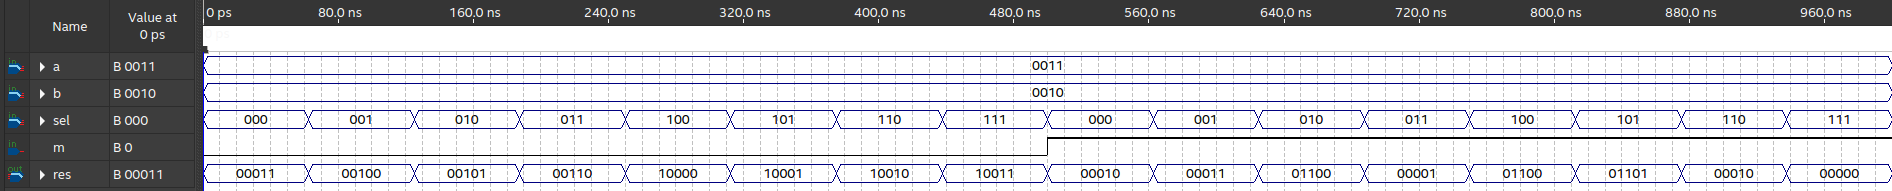
\includegraphics[width=\textwidth]{inciso-b-sim}
  \caption{Simulación del circuito (Parte B)}
  \label{fig:inciso_b_sim}
\end{figure}

\subsubsection*{Funcionamiento en la tarjeta de desarrollo}
Haciendo uso de una correcta asignación de pines en la sección de \textit{Pin 
Planner}, se puede cargar el programa a la tarjeta a través del modo 
\textit{Programmer}.

Se tomaron foto de algunos algunos casos de pueba significativos y referentes 
a la simulación de la Figura \ref{fig:inciso_b_sim}. El primero que se tiene 
es el de $sel(2) = 0$, $sel(1) = 0$ y se varían $sel(0)$ y $m$.
\begin{figure}[H]
  \centering
  \begin{subfigure}[b]{0.45\textwidth}
    \centering
    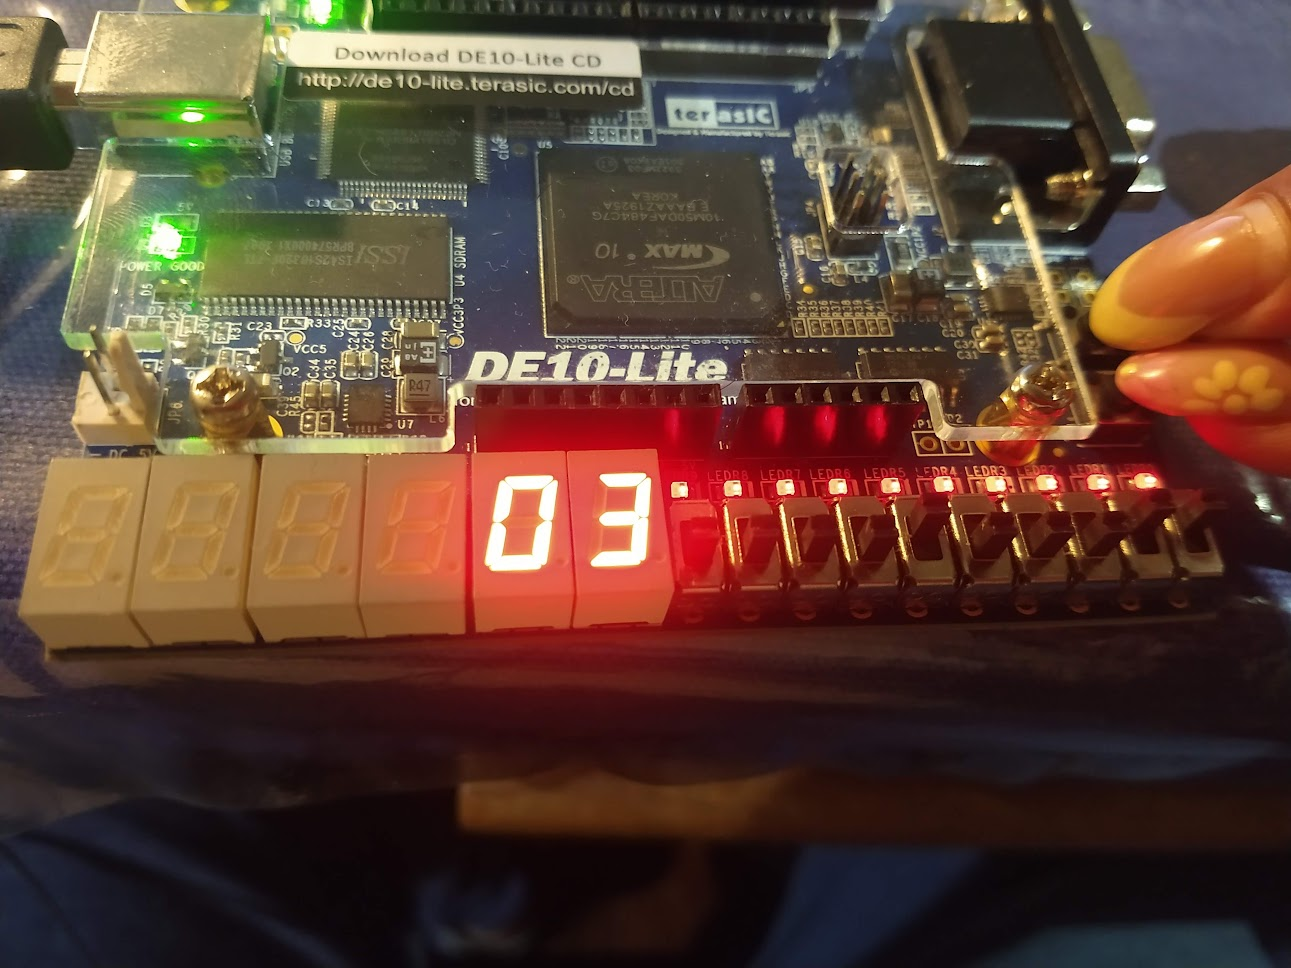
\includegraphics[width=\textwidth]{ej_0000}
    \caption{Caso de prueba $sel = 000$, $m = 0$}
    \label{fig:b_tarj_1}
  \end{subfigure}
  \begin{subfigure}[b]{0.45\textwidth}
    \centering
    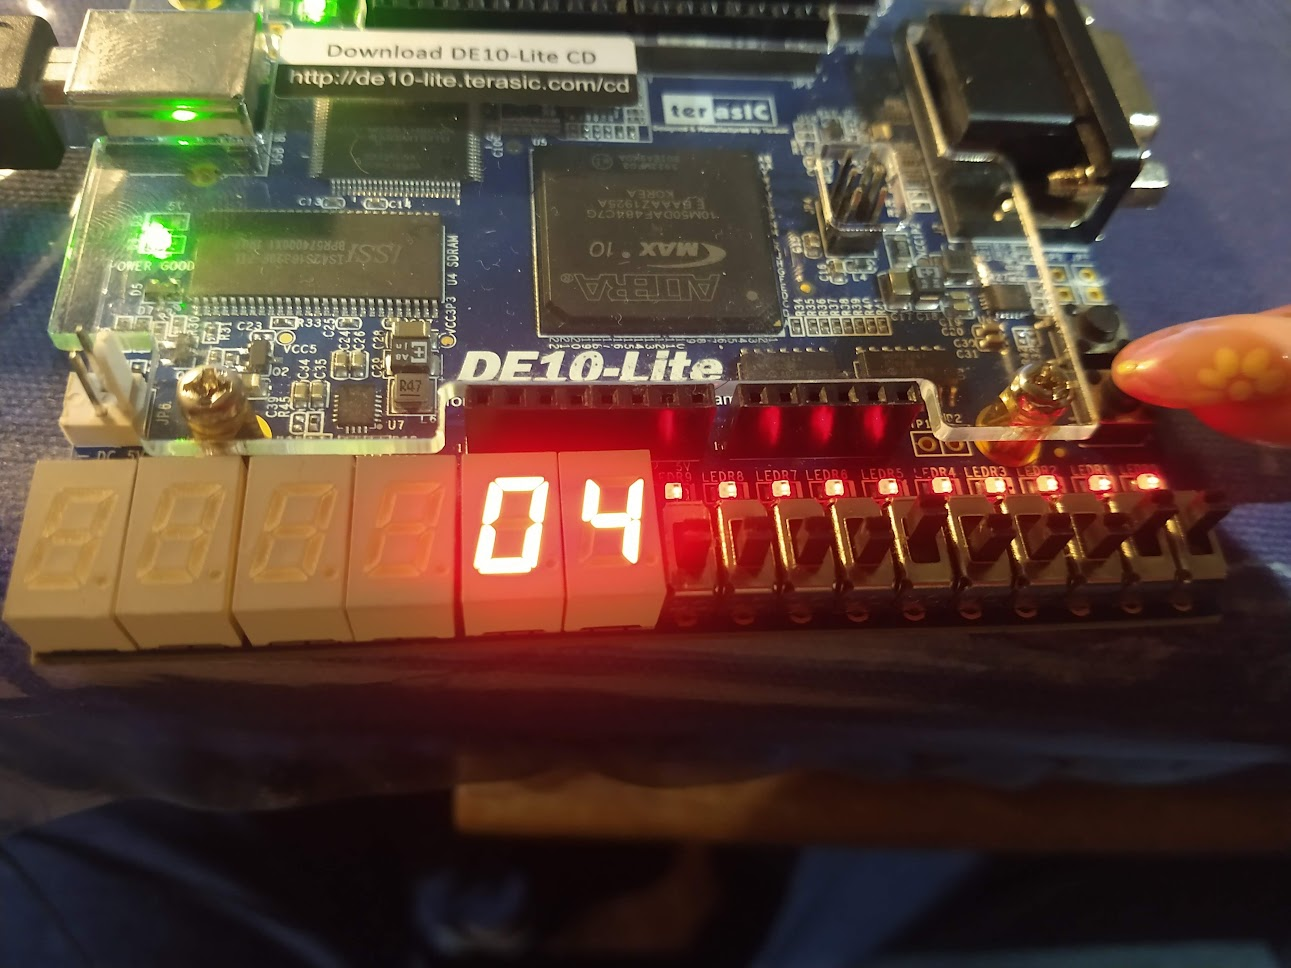
\includegraphics[width=\textwidth]{ej_0010}
    \caption{Caso de prueba $sel = 001$, $m = 0$}
    \label{fig:b_tarj_2}
  \end{subfigure}
  \begin{subfigure}[b]{0.45\textwidth}
    \centering
    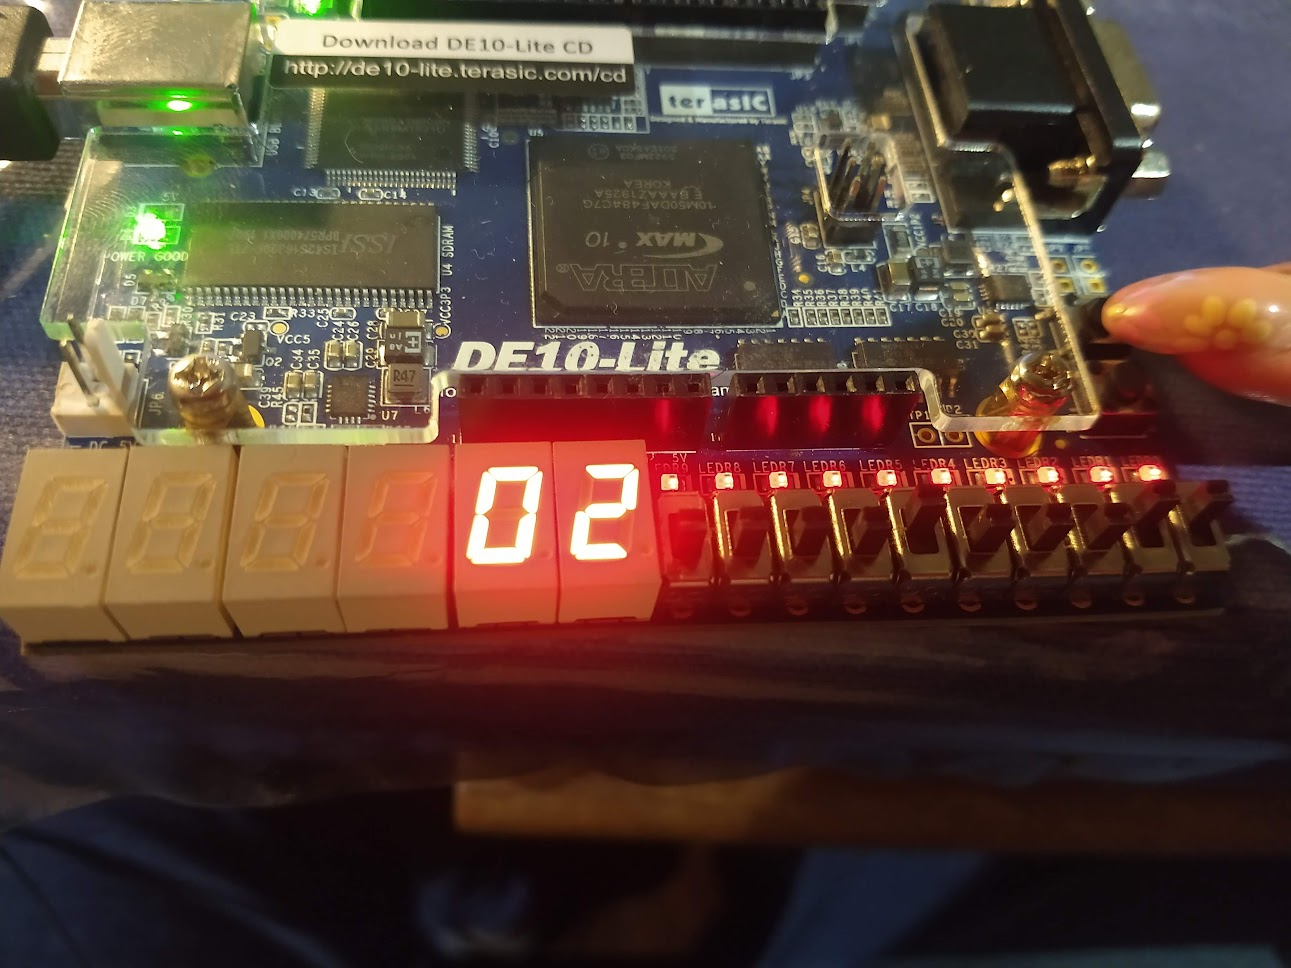
\includegraphics[width=\textwidth]{ej_0001}
    \caption{Caso de prueba $sel = 000$, $m = 1$}
    \label{fig:b_tarj_3}
  \end{subfigure}
  \begin{subfigure}[b]{0.45\textwidth}
    \centering
    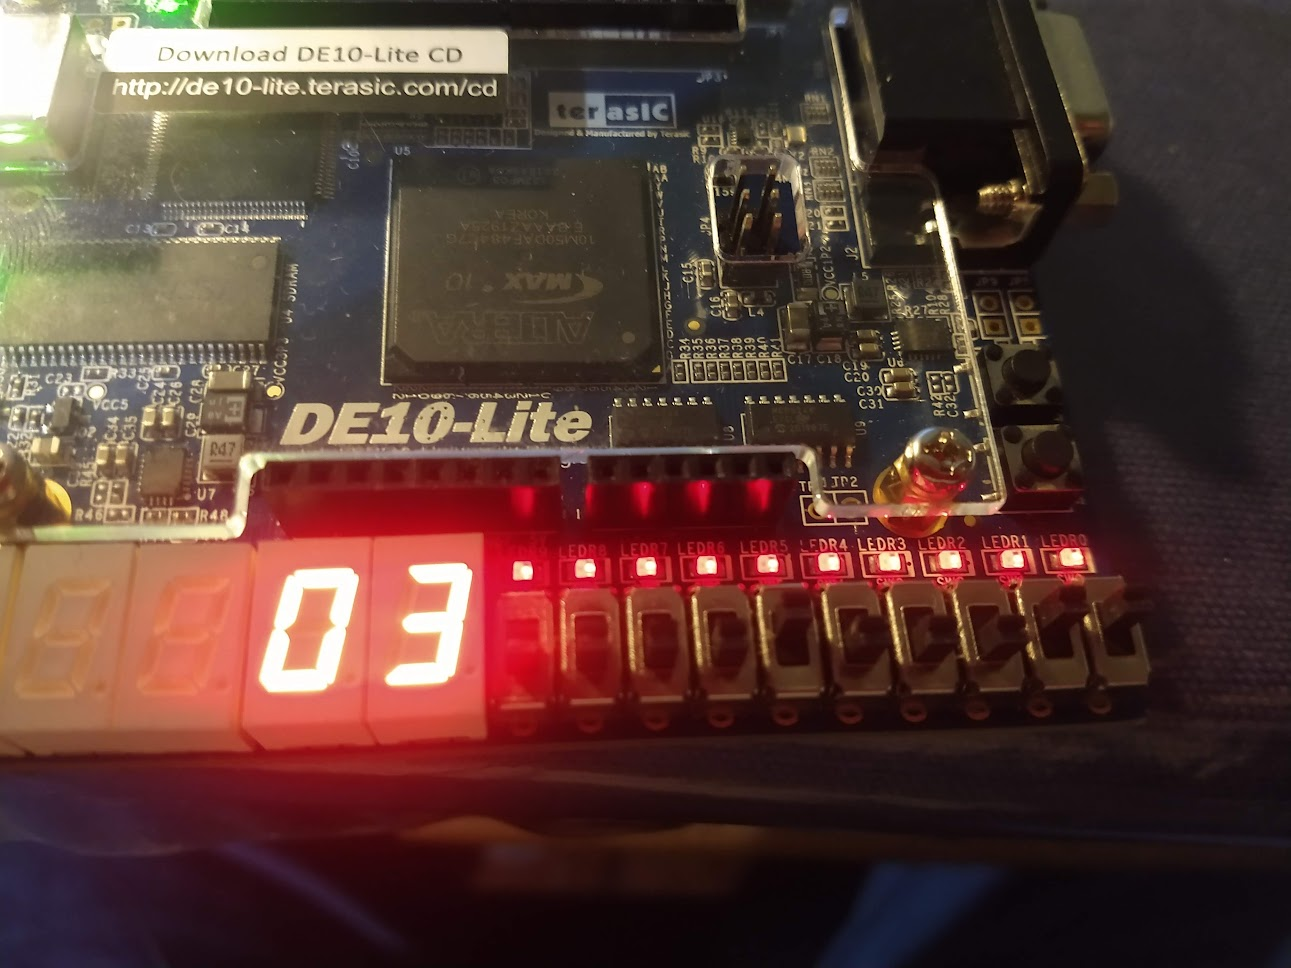
\includegraphics[width=\textwidth]{ej_0011}
    \caption{Caso de prueba $sel = 001$, $m = 1$}
    \label{fig:b_tarj_4}
  \end{subfigure}
  \caption{Primer caso de prueba (Sección B)}
\end{figure}

Los resultados coinciden con la simulación (tomando en cuenta el hexadecimal, 
claeramente). Se realizó otro caso de prueba adicional para tener en 
consideración más posibilidades. El caso $sel(2) = 1$, $sel(1) = 0$ y se 
varían $sel(0)$ y $m$.
\begin{figure}[H]
  \centering
  \begin{subfigure}[b]{0.45\textwidth}
    \centering
    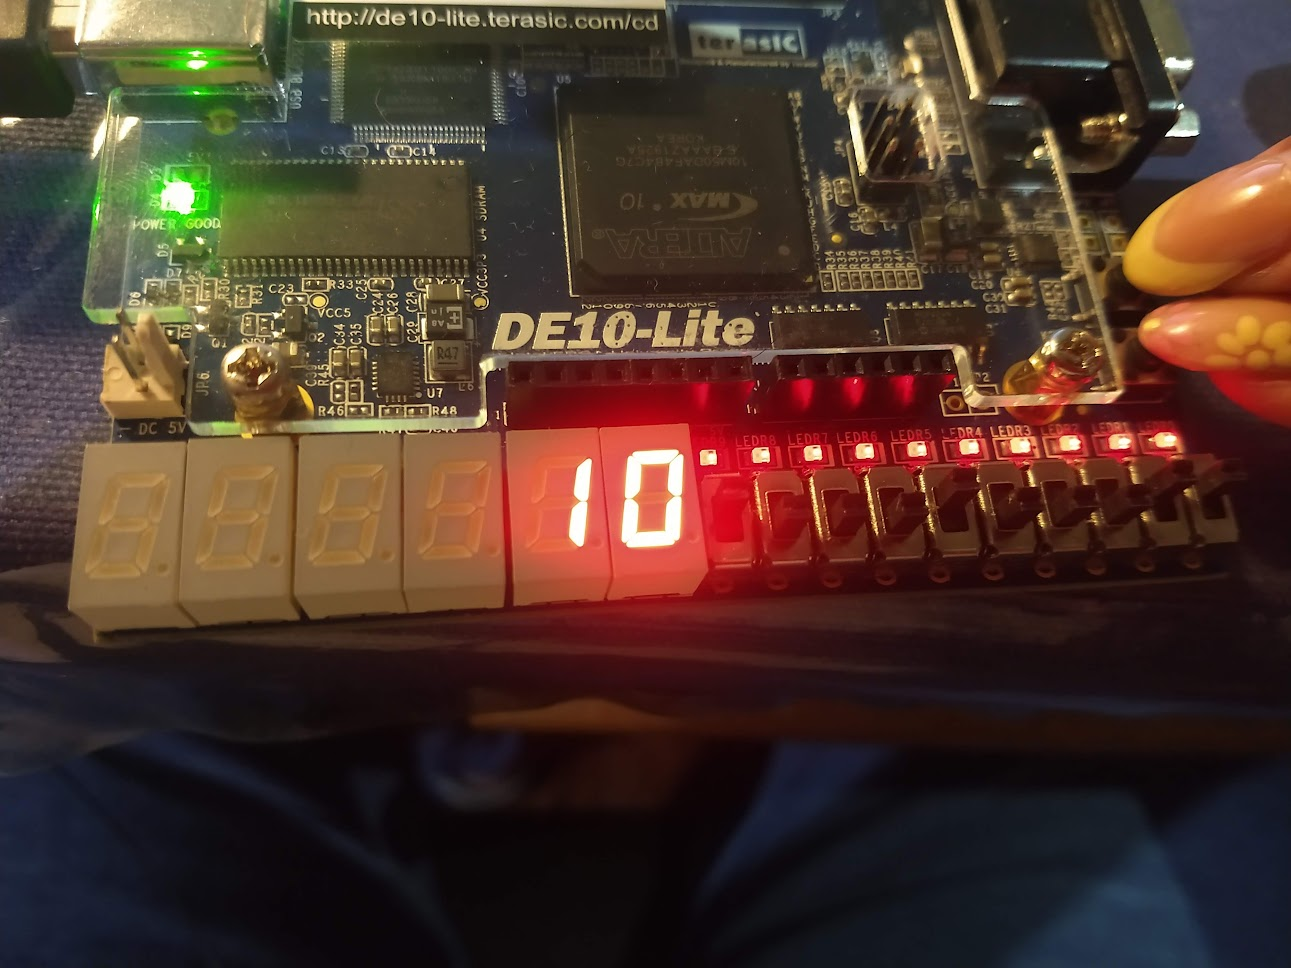
\includegraphics[width=\textwidth]{ej_1000}
    \caption{Caso de prueba $sel = 100$, $m = 0$}
    \label{fig:b_tarj_5}
  \end{subfigure}
  \begin{subfigure}[b]{0.45\textwidth}
    \centering
    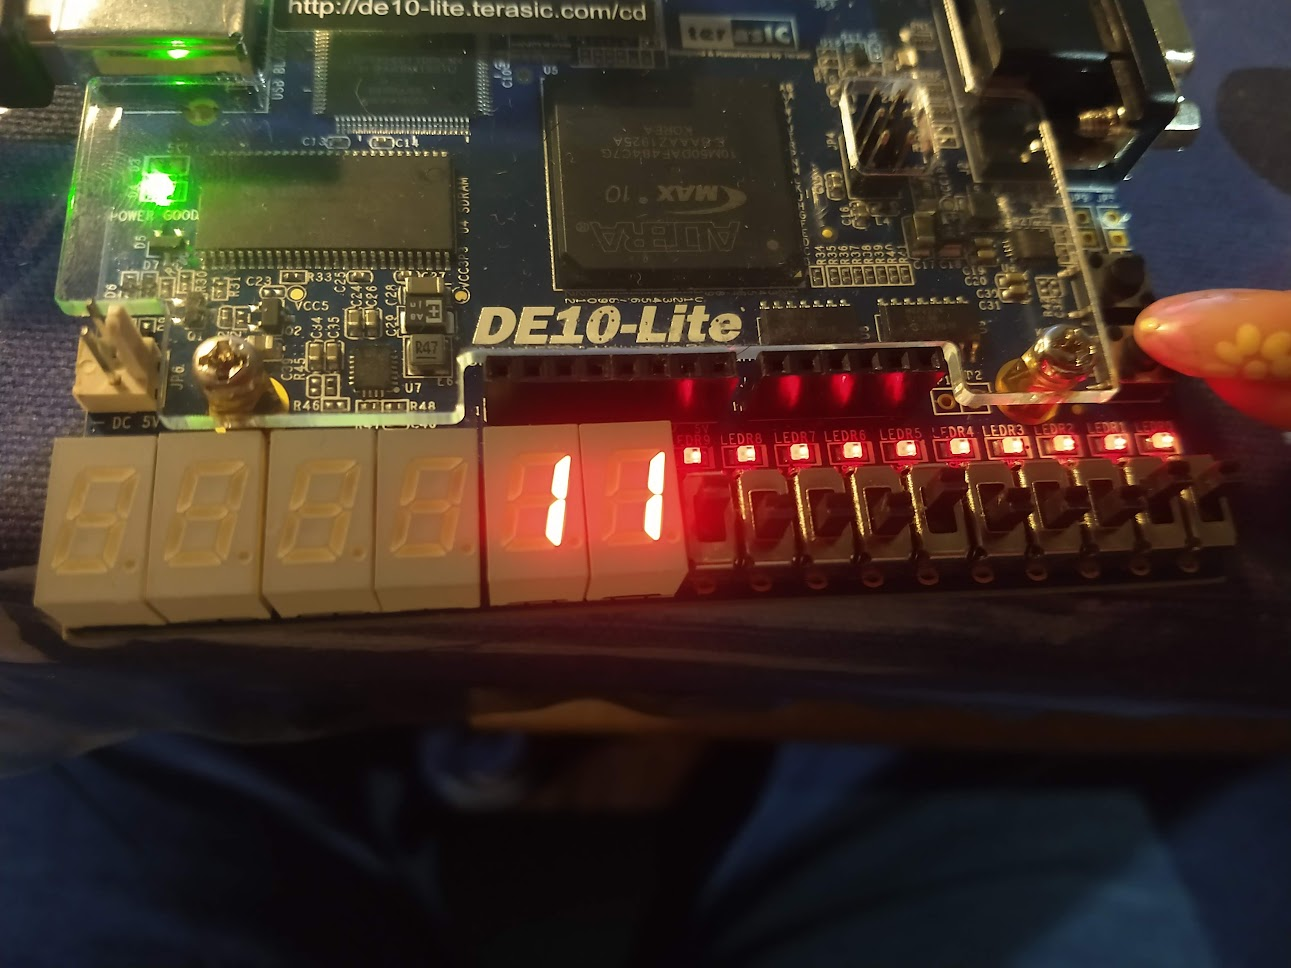
\includegraphics[width=\textwidth]{ej_1010}
    \caption{Caso de prueba $sel = 101$, $m = 0$}
    \label{fig:b_tarj_6}
  \end{subfigure}
  \begin{subfigure}[b]{0.45\textwidth}
    \centering
    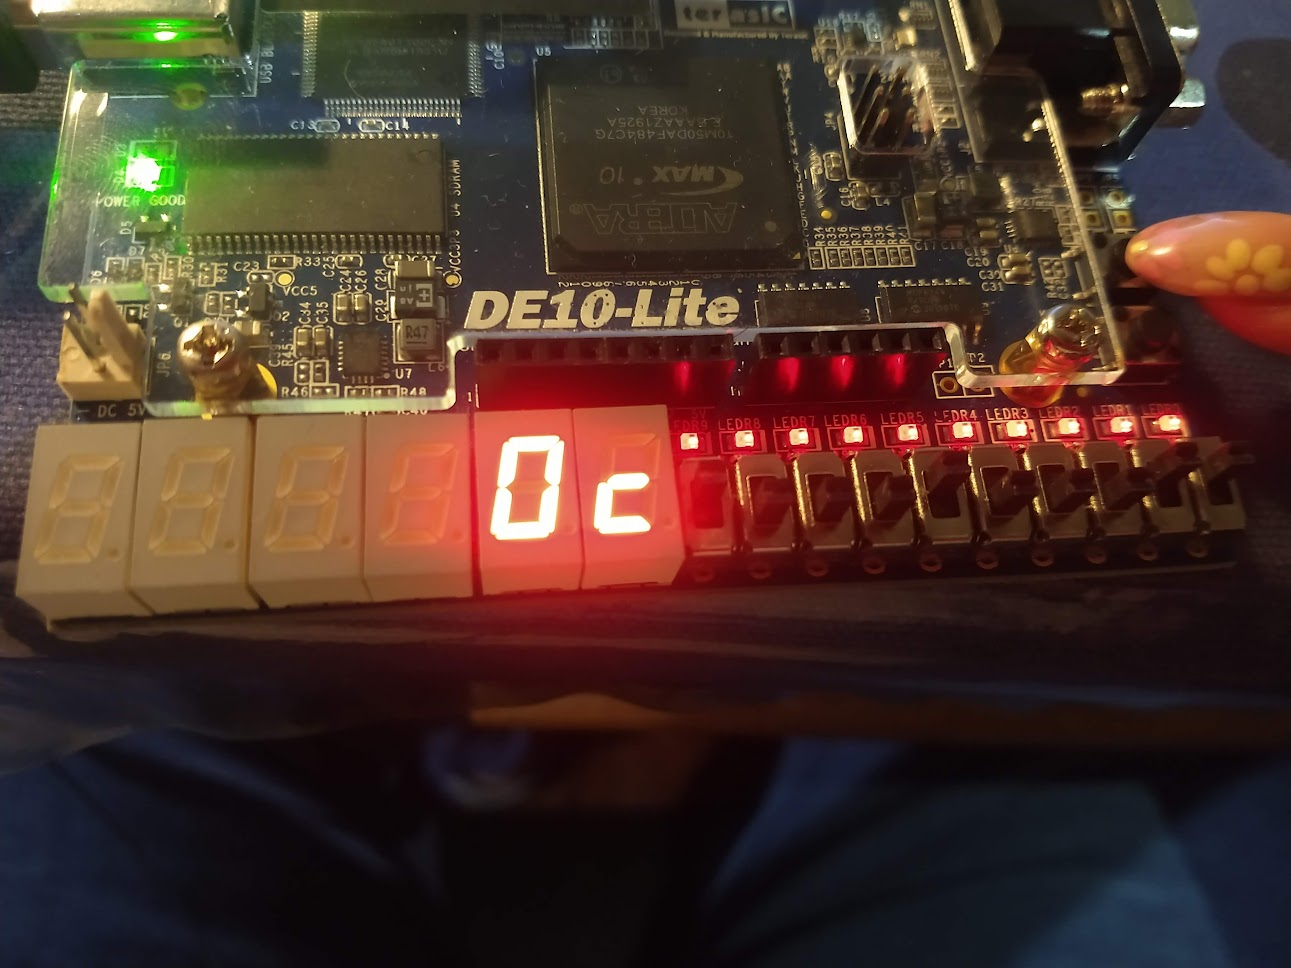
\includegraphics[width=\textwidth]{ej_1001}
    \caption{Caso de prueba $sel = 100$, $m = 1$}
    \label{fig:b_tarj_7}
  \end{subfigure}
  \begin{subfigure}[b]{0.45\textwidth}
    \centering
    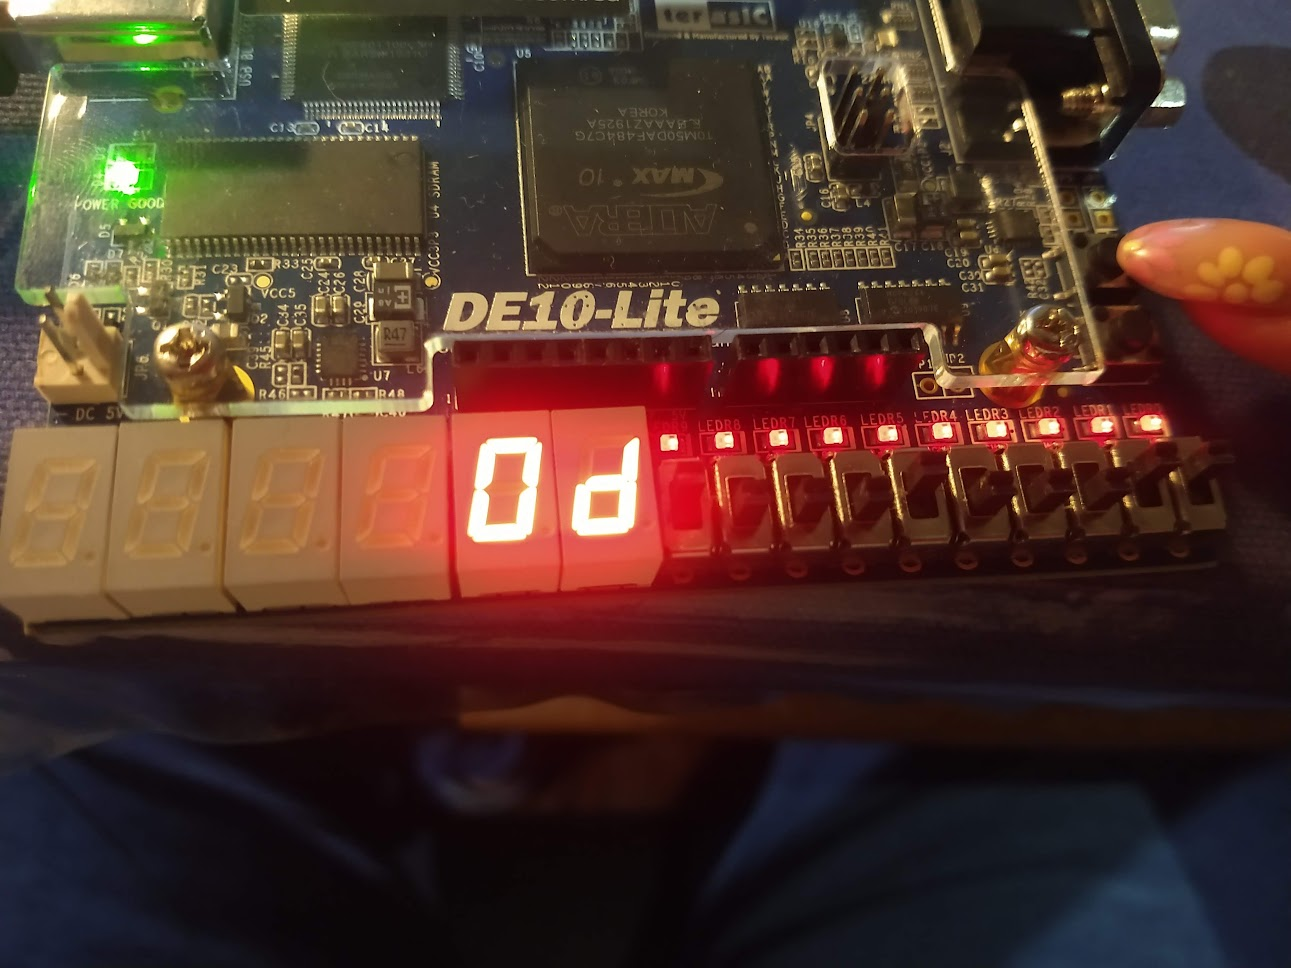
\includegraphics[width=\textwidth]{ej_1011}
    \caption{Caso de prueba $sel = 101$, $m = 1$}
    \label{fig:b_tarj_8}
  \end{subfigure}
  \caption{Segundo caso de prueba (Sección B)}
\end{figure}

Nuevamente, los resultados coinciden con los de la Figura 
\ref{fig:inciso_b_sim}, con lo cual se puede concluir que el problema se 
solucionó de forma exitosa.


\end{document}
